\documentclass[a4paper, 11pt]{article}

\voffset -0cm
\hoffset 0.0cm
\textheight 23cm
\textwidth 16cm
\topmargin 0.0cm
\oddsidemargin 0.0cm
\evensidemargin 0.0cm

\usepackage[ruled,vlined,linesnumbered]{algorithm2e}   % authors: last version of algorithm display

\usepackage{epsfig}
\usepackage{setspace}
\usepackage{fancyheadings}
\usepackage{amsmath}
\usepackage{amssymb}
\usepackage{graphicx}
\usepackage{url}
\newtheorem{Lemma}{Lemma}

\title{}
\author{}
\date{}

\newtheorem{qu}{Question}

\begin{document}

\begin{center}
	\LARGE \textbf{Assignment: ``Images et g\'eom\'etrie discr\`ete''}
\end{center}

\section*{Introduction}

The objective of this project is to perform experimental evaluation of
multigrid behavior of differential estimators. This project is based
on practical-work TP6 and TP7.

We expect from you:
\begin{itemize}
\item A short report with answers to the "formal" questions and
  description of the your implementations choices (Sect. 2)
\item A C++ project (\texttt{CMakeLists.txt} plus couple of
  \textbf{commented} cpp program files).
\end{itemize}




\section{Multigrid analysis of Maximal Segments}

We would like to evaluate experimentally the behavior of maximal
segments in a multigrid framework. More precisely, we would like to
evaluate the following quantities:
\begin{itemize}
\item The number of maximal segments.
\item The max/min values of maximal segment lengths.
\item The average length of maximal segments.
\end{itemize}

More precisely, we can to evaluate the following statement:

\begin{Lemma}[Asymptotic Laws of Maximal Segments]
  \label{lem-asymptotic-digital-length-ms}
   Let $X$ be some convex shape of $\mathbb{R}^2$, with at least
   $C^3$-boundary and bounded curvature.  The discrete length (number
   of points) of
   maximal segments in $\partial Z$ for $Z=Dig(X,h)$ follows:
   \begin{itemize}
   \item the shortest is lower bounded by
     $\Omega(h^{-\frac{1}{3}})$;
   \item the longest is  upper bounded by
     $O(h^{-\frac{1}{2}})$;
   \item their average length, denoted $L_D({Z})$, is
     such that:
  \begin{equation}
    \label{eq:lengthMS}
    \Theta(h^{-\frac{1}{3}}) \le L_D( {Z} ) \le \Theta(h^{-\frac{1}{3}} \log \left(\frac{1}{h}\right))\;.
  \end{equation}
   \end{itemize}
\end{Lemma}


\begin{qu}
  Implements a piece of code that first consider multigrid
  digitization of an Euclidean convex object (e.g. sphere or ellipse
  from implicit equation) and extract its contour. Perform a complete
  maximal covering of the contour into maximal DSS.
\end{qu}


\begin{qu}
  Perform a complete multigrid analysis to verify Lemma 1: statistics
  of the maximal segment length distribution, behavior (graphs) when
  $h$ tends to 0...
\end{qu}


\begin{qu}
  Can you conclude something on the probability, for spheres or
  ellipses,  that maximal segment have pathological
  $O(h^{-\frac{1}{2}})$ length cases ? For a fixed resolution, where
  those pathological cases are located on the contour ?
\end{qu}


\begin{qu}
  Consider now digitization of implicit non-convex shapes (please
  consider a non-convex shape with various inflection points). Is
  Lemma 1 still valid ?
\end{qu}



\section{Extended Euclid's Algorithm}

Let us consider the following Euclidean division algorithm.

\begin{procedure}[H]
\caption{Convergents( $\text{(a,b), (p,q), (p',q'), i}$ )}
\label{algo:conv}
\KwIn{$(a,b)$, $(p,q)$, $(p',q')$, $i$}
\KwOut{$(p',q')$}
%
Let $r$ be the remainder of the Euclidean division $b/a$\;
Let $u$ be the quotient  of the Euclidean division $b/a$\;
$p'' \leftarrow up' + p$\; $q'' \leftarrow uq' + q$\;
\eIf{$r > 0$}{
 \Return{Convergents($(r,a)$, $(p',q')$, $(p'',q''), i+1$)}\;
}{
 \Return{$(p',q')$}
}
\end{procedure}


\begin{qu}
\label{qu:init}
  Let $(p_{-1},q_{-1})=(1,0)$ and $(p_0,q_0)=(0,1)$, what is the
  output of \emph{\texttt{Convergents}}($(5,8)$, $(p_{-1},q_{-1})$,
  $(p_0,q_0)$, 0) ?
\end{qu}


\begin{qu}
  Let us consider \emph{\texttt{Convergents}}($(a,b)$, $(p_{-1},q_{-1})$,
  $(p_0,q_0)$, 0) (with $0 \leq a < b$ and $\gcd{(a,b)} = 1$). We
  index the recursive calls by $i=1\ldots n$. Show that
  \begin{displaymath}
    \forall i=1\ldots n\,, p_i=u_ip_{i-1}+p_{i-2}\text{ and } q_i=u_iq_{i-1}+q_{i-2}\,.
  \end{displaymath}
\end{qu}


\begin{qu}
Similarly, with $r_{-1}=b$ and $r_0=a$, show that
  \begin{displaymath}
    \forall i=1\ldots n\,, r_i=r_{i-2}- u_ir_{i-1}
  \end{displaymath}
\end{qu}

\begin{qu}
  Following previous results, prove the following statements:

  \begin{enumerate}
  \item $\forall i=1\ldots n\,, p_{i-1}q_i - q_{i-1}p_i = \pm 1$
  \item $\forall i=-1\ldots n\,, p_{i}b - q_{i}a = \pm r_i$
  \end{enumerate}
Since $r_n=gcd(a,b)=1$, what is $p_nb-q_na$ ?
\end{qu}

\begin{qu}Give the definition of uni-modularity. What is the
  geometrical interpretation of this definition ?
\end{qu}


\begin{qu}
  In the domain in appendix\footnote{Please checkout the git project
    to get the PDF file of the figure.}}, draw the Euclidean segment
  $[(0,0)-(b,a)]$ and all convergents $(q_i,p_i)$ for the input given
  in Question \ref{qu:init}. With respect to the parity of $i$, can
  you say something on the position of convergents with respect to the
  segment ? If we construct a polygonal curve with only convergents
  $(q_i,p_i)$ with even index $i$ (plus a last point $(b,a)$). What
  kind of geometrical object I have constructed ?
\end{qu}


\begin{qu}
  Let $L_{odd}$ (resp. $L_{even}$) be the polygonal curve of convergents with
  odd index (resp. even index). Furthermore, we add the point $(b,a)$
  to the end of each list. For the input given in Question
  \ref{qu:init}, are there integer points between $L_{odd}$ and
  $L_{even}$ ? Why ?
\end{qu}


\begin{qu}
  For a general setting \emph{\texttt{Convergents}}($(a,b)$, $(p_{-1},q_{-1})$,
  $(p_0,q_0)$, 0), can you prove the statement of the previous
  question ?
\end{qu}

\begin{qu}
  What is the complexity of \emph{\texttt{Convergents}} with respect
  to $a$ and $b$ ?
\end{qu}





\newpage
\appendix

\begin{center}
  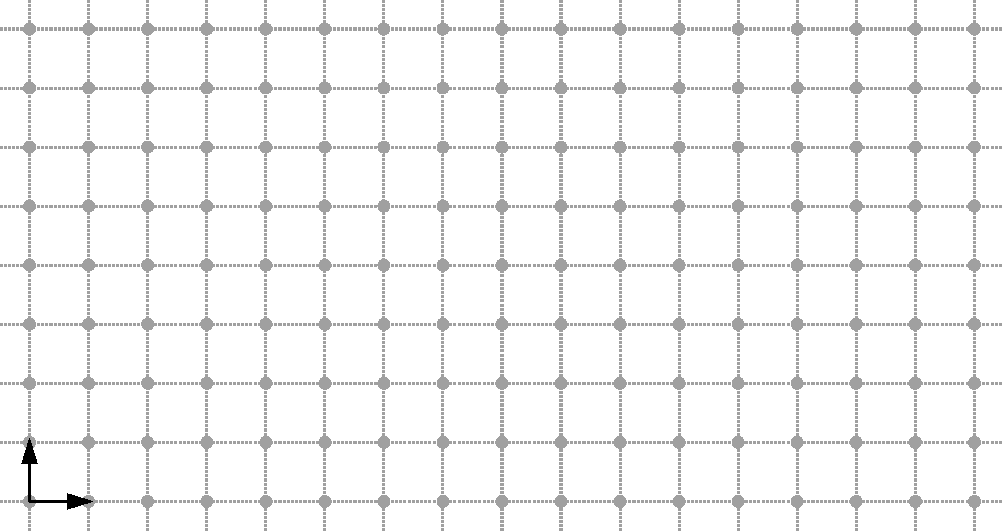
\includegraphics[width=8cm]{domain}
\end{center}


\begin{center}
  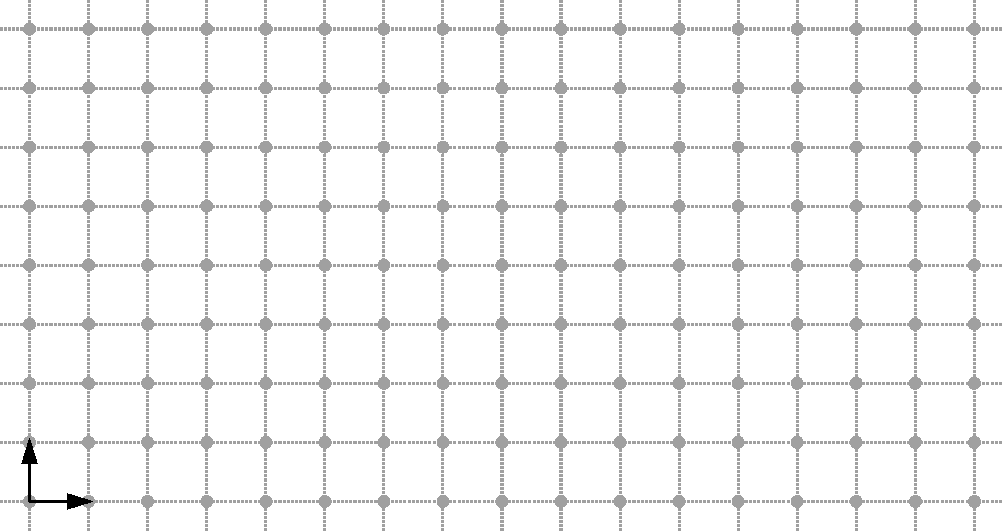
\includegraphics[width=8cm]{domain}
\end{center}


\end{document}
